\newpage
\subsubsection{Caso d'uso UC4.4: Login tramite LinkedIn }
\label{UC4_2}
\begin{figure}[!htbp]
	\centering
	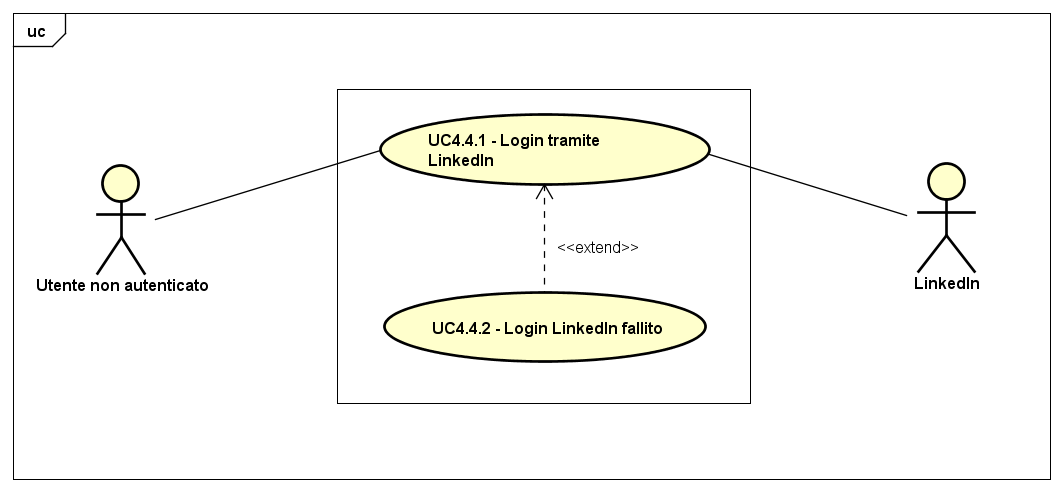
\includegraphics[scale=0.45]{UML/UC4_4.png}
	\caption{UC4.2: Login tramite LinkedIn}
\end{figure}

\begin{tabular}{ l | p{11cm}}
	\hline
	\rowcolor{Gray}
	\multicolumn{2}{c}{UC4.4 - Login tramite LinkedIn} \\
	\hline
	\textbf{Attori} & Utente non autenticato, LinkedIn \\
	\textbf{Descrizione} & L'attore Utente non autenticato effettua il login all'applicazione web tramite LinkedIn, così da evolversi in un utente autenticato\\
	\textbf{Pre-Condizioni} & L'attore Utente non autenticato ha scelto di eseguire il login all'applicazione web e non è autenticato \\
	\textbf{Post-Condizioni} & L'attore Utente non autenticato ha effettuato il login all'applicazione web tramite LinkedIn, evolvendosi in un utente autenticato \\
	\textbf{Scenario Principale} & \begin{enumerate*}[label=(\arabic*.),itemjoin={\newline}]
		\item L'attore effettua il login con successo tramite LinkedIn, evolvendosi in un Utente autenticato (UC2)
	\end{enumerate*}\\
	\textbf{Scenari Alternativi} & \begin{enumerate*}[label=(\arabic*.),itemjoin={\newline}]
		\item L'attore ha fallito il login tramite LinkedIn (E.g: Mancanza di privilegi e autorizzazioni, utente non loggato correttamente a LinkedIn)
	\end{enumerate*}\\
\end{tabular}